\documentclass[../main.tex]{subfiles}
\graphicspath{{\subfix{../src/}}}


\begin{document}
\section{Problem Specification}

There is a large need for new technology that improves the effectiveness and ergonomics of human hand prosthetics.
Current state-of-the-art prosthetic products on the market exhibits a severe reduction of controllable degrees of Freedom compared to their biological counterparts.
Some prosthetics products are simple in design, often using a small set of motors to control multiple joints at the same time, furthermore, these products often rely on simple, grasp control based on 2 or more \gls{sEMG} interfaces.
These \gls{sEMG} interfaces are used to classify ``open/close'' signals generated by the muscles in the residual limb of the amputee.
The prosthetics user is manually required to change control-scheme between different grip typs, creating very crude control dynamics that is fundamentally different from biological hand control.

\begin{figure}[H]
\begin{center}
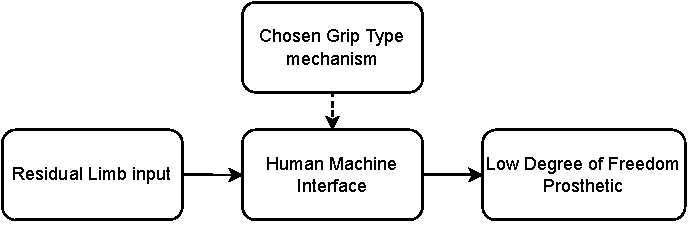
\includegraphics[width=0.8\textwidth]{NonIdealProsthetic.pdf}
\caption{Example of a current commercial prosthetic control scheme.}
\label{fig:nonidealprosthetic}
\end{center}
\end{figure}

%TODO: I need examples to back up my slander of modern *commercial* prosthetics!
% Maybe explain they need to be like this to be robust, and that research methods are not robust enough yet to be commercial?

%A in-debth explanation of ``open/close'' control can be seen in section \ref{???}
%TODO: This sounds weird, integrate a simple controller therory here, and why it is so crude, then refrence it in state-of-the-art
%TODO: Create refrence
Crude controllability of upper-limb prosthetics is a great pitfall in the field of research and development of prosthetics, this has a large impact on rehabilitation of amputees.
The World Health Organization (WHO) defines rehabilitation as ``a set of interventions designed to optimize functioning and reduce disability in individuals with health conditions in interaction with their environment'' \cite{WHO_rehab}.
Proper rehabilitation and function of the prostetic is crucial to the independence of the amputee, but unsatisfactory function of prosthetics lead to amputees, that exhibit a great deal of stress during the rehabilitation process.
Insatisfaction and stress can cause the patient to repel the rehabilitation process and the prosthetic all-together \cite{Kristin2012}.
The repelling of the prostetic increase in the cases of the most severe cases of amputation, where the largest amount of control muscles are lost.
These amputations are often located further up the limbs, where the loss of mobility and controllability are greatest.
The type of prosthetic the amputee is able to recieve is highly dependent on the severity of the loss of limb, furthermore, the amount of muscles leftover from amputation also dicates the type of prosthetic interface the patient is able to interface with.
%TODO: Refrence for this!
Patients of hand amputation are able to recieve prosthetics with much more control of individual movements due to the muscles controlling the lost limb being intact. 
Lower-arm amputation patients has less control over their prosthetic due to the loss of the muscles in the lower-arm.
%TODO: Tech2015 can be a good ref for state-of-the-art stuff 
The differences between severity is a problem in prosthetics design because it is impossible to create a standardized prosthetic that suits most patient's needs.



%TODO: This one is bad
%State-of-the-art commercial prosthetics further decrease the controllable DoF in order to increase robustness of the control experience, this is further elaborated upon in \ref{sec:stateoftheart}.
%TODO: Create refrence for state-of-the-art

%TODO: Problem specification should be an entire page!
\newpage
\subsection{Motivation}


\begin{figure}[h]
\begin{center}
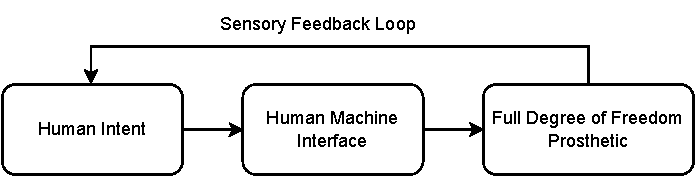
\includegraphics[width=0.8\textwidth]{IdealProsthetic.pdf}
\caption{The Ideal design of a prosthetic device.}
\label{fig:idealprosthetic}
\end{center}
\end{figure}



This thesis aims to summarize, and compare current state-of-the-art research and products in the field of prostetics devices, and products the control of prosthetics and the existing limitations of these state-of-the-art products. 
This thesis aims to contribute to the world of prosthetics control, by researching effective methods of collecting sensory data from the lower-/upper-arm, and by doing so, creating an state-of-the-art Artificial Intelligence (AI) based controller, that is able to imitate the intent and movements or a real hand.
And by doing so, by improving sEMG controller design to increase functionality and the controllable DoF of the prosthetic, to provide a more true-to-life experience to the prosthetics user, and thus reduce the amount of patients that disregard prosthetics.
This thesis also aims to explore efficient methods of designing a network to identify lower-/upper-arm muscolatory intent, with the purpose of controlling a simulated prosthetics device, and by doing so, increase the controllable Degree-of-Freedom for the prostetics user.


The main goal of this thesis is to provide a meaningful contribution to the world of prosthetics design and control.
In order to confine the workload done in this thesis, a set of development goals has been made:

%TODO: Refer to these in the report! make it the key motivations for all my choises.
\begin{enumerate}
\item Create a software-based, biology-inspired, anatomically realistic simulation of a humanoid lower-arm/hand that is able to imitate the movements of the humanoid limb.
\item Make the prosthetics simulation controllable from a widely-used robotics-software.
\item Design a sEMG muscle pre-prossesing pipeline for a prosthetics controller. 
\item Design a state-of-the-art prosthetics controller based on AI, to control a simulated prosthetics device.
\item Create a custom dataset to train AI based controllers for prosthetics.
\item Test and Validate the created prosthetics controller against state-of-the-art methods.
\end{enumerate}
%TODO: This needs


\end{document}
